\documentclass[../Notes.tex]{subfiles}

\begin{document}

    \NewDocumentCommand{\codeword}{v}{
        \texttt{\textcolor{blue}{#1}}
    }

     \subsection*{(\S 1.2) Descriptive statistics; (\S 1.3) Measures of location}

    Common naming conventions:
    \begin{itemize}
        \item Population size: $N$
        \item Sample size: $n$
        \item Sample from two different populations: $n, m,$ or $n_1, n_2$
        \item Data: $x_1, x_2, x_3, \dots x_n$
    \end{itemize}

    \subsubsection{Stem-and-leaf displays}

\begin{lstlisting}[language=R]
    > x sample(1:50, size=20, replace=TRUE)
    > sort(x)
    [1] 2 2 2 3 9 14 18 19 20 21 21 22 22 29 30 32 32
    [18] 33 44 47
    > stem(x)
\end{lstlisting}

    The sample function generates numbers in the range provided as the first argument, with a size equal to the second argument. sort(x) sorts the values stored in x, and stem(x) does the following:

    Each ``stem'' refers to the highest digits and each ``leaf'' is the latter digits. This is the stem-and-leaf display for the dataset stored in x:

    \begin{center}
        \resizebox{0.35\hsize}{!}{
            \begin{tabular}{r | l}
                Stem & Leaves       \\
                \hline              
                0 & 2 2 2 3 9       \\
                1 & 4 8 9           \\
                2 & 0 1 1 2 2 9     \\
                3 & 0 2 2 3         \\
                4 & 4 7
            \end{tabular}
        }
    \end{center}

    \subsubsection{Dot plots}
\begin{lstlisting}[language=R]
    > x <- sample(1:10, size=15, replace=TRUE)
    > x
    [1] 7 8 1 3 4 10 1 2 2 1 1 4 4 9 6
    > stripchart(x, method="stack", offset=0.5, at=0.15, pch=20)
\end{lstlisting}

    \codeword{stripchart()} constructs the dot plot. The \codeword{offset} and \codeword{at} values affect the appearance. \codeword{pch} means \codeword{p}rinting \codeword{ch}aracter. Having it set to 20 makes the dot solid.

    \begin{center}
        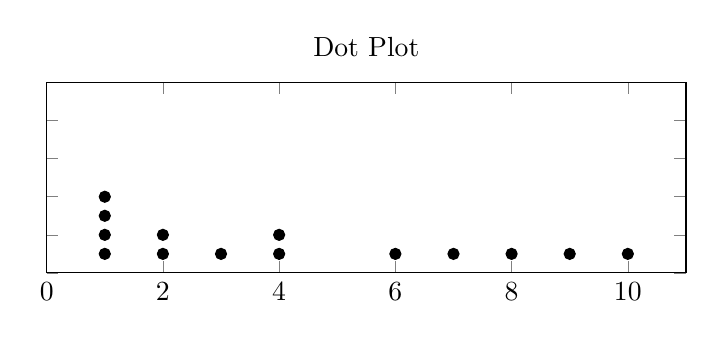
\begin{tikzpicture}
            \begin{axis}[
                title={Dot Plot},
                xmin=0, xmax=11,
                ymin=0, ymax=10,
                yticklabels={},
                width=0.8\textwidth,
                height=4cm
            ]
            
            \addplot[only marks, scatter src=explicit symbolic
                ]
                table[row sep=\\] {
                    x y \\
                    1 1 \\
                    1 2 \\
                    1 3 \\
                    1 4 \\
                    2 1 \\
                    2 2 \\
                    3 1 \\
                    4 1 \\
                    4 2 \\
                    6 1 \\
                    7 1 \\
                    8 1 \\
                    9 1 \\
                    10 1\\
                };
                
            \end{axis}
        \end{tikzpicture}
    \end{center}

    \subsubsection{Histograms}

    \begin{itemize}
        \item For quantitative data.
        \item May differ depending on whether a variable is discrete or continuous.
    \end{itemize}

    \textbf{Discrete} data is either infinite or countably infinite: orderable, typically integers. Includes ration numbers.

    \begin{itemize}
        \item $x_1$ = \# of tuberculosis cases in the 50 largest U.S. cities in 2013. $\leftarrow$ Might be 0, 1, 2, \dots but $\neq \infty$.
        \item $x_i$ \# of ``successes'' when 100 patients treated. $\leftarrow$ Count data in which we know a hard upper limit (in this case 100).
        \item $x_i$ \# of rooms in a rental unit. $\leftarrow$ 1, 2, \dots, 100. At least 1 guaranteed as a hard minimum limit.
    \end{itemize}

    Histograms, when data is discrete, use vertical bars with height proportional to the number of times each value occurs.

    \begin{center}
        Frequency Histogram vs Relative Frequency Histogram

        For the data: $\{1, 1, 2, 2, 2, 3\}$
    
        \begin{figure*}[h]
            \centering
            \begin{minipage}[h]{.45\linewidth}
                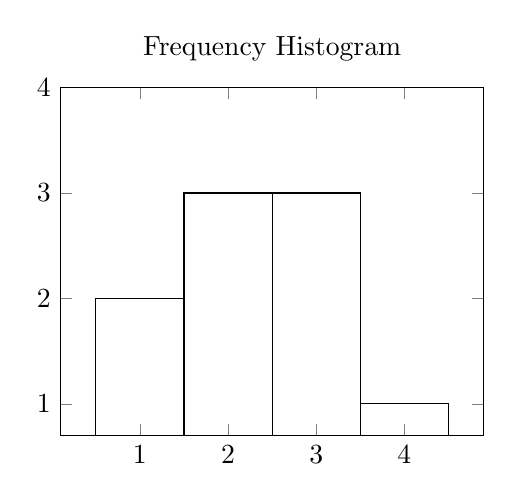
\begin{tikzpicture}
                    \begin{axis}[title={Frequency Histogram}, ymax=4, area style, height=6cm]
                        \addplot[ybar interval, mark=no] coordinates { (0.5, 2) (1.5, 2) (1.5, 3) (2.5, 3) (3.5, 1) (4.5, 1) };
                    \end{axis}
                \end{tikzpicture}
            \end{minipage}
            \begin{minipage}[h]{.45\linewidth}
                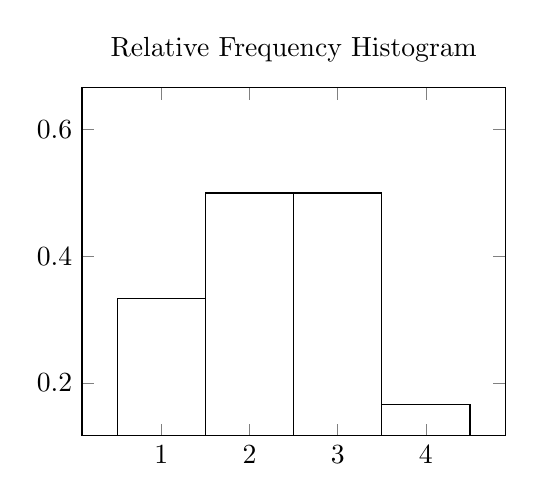
\begin{tikzpicture}
                    \begin{axis}[title={Relative Frequency Histogram}, ymax=0.666, area style, height=6cm]
                        \addplot[ybar interval, mark=no] coordinates { (0.5, 1/3) (1.5, 1/3) (1.5, 1/2) (2.5, 1/2) (3.5, 1/6) (4.5, 1/6) };
                    \end{axis}
                \end{tikzpicture}
            \end{minipage}
        \end{figure*}
    \end{center}

    Relative Frequency Histograms have a total height of 1.

    \pagebreak

    \subsubsection{R Code for Histograms}

\begin{lstlisting}[language=R]
    > # Use R to simulate 100 values from {1, 2, 3, ..., 10}
    > my_data <- sample(1:10, size=100, replace=TRUE)
    > # Here are the first 20 values:
    > my_data[1:20]
    [1] 4 3 5 6 5 4 10 2 6 2 5 8 7 10 4 10 7 6
    [19] 5 7
    > # Create a frequency histogram:
    > hist(my_data. main="Plot 1 - discrete data")
    > # Create a relative frequency histogram:
    > hist(my_data, probability=TRUE, main="Plot 2")
\end{lstlisting}

\emph{Note: R uses \# for comments. You're a CS major, you know what these functions and their arguments do.}

\subsubsection{R Code of a Histogram Using Continuous Data}

\begin{lstlisting}[language=R]
    > # Generate 100 rational values from 1:10.
    > my_data <- runif(100, min=1, max=10)
    > # Create a histogram using the same code for discrete data:
    > hist(my_data, main="Plot 3 - Continuous Data")
    > # And a relative frequency histogram:
    > hist(my_data, probability=TRUE, main="Plot 4")
\end{lstlisting}

    Here, \codeword{r} refers to random and \codeword{unif} refers to uniform in \codeword{runif}, it does not refer to \codeword{run} \codeword{if}.

    \subsection*{(\S 1.3) Measures of Location}

    There are several ways to measure where the center of a data set s. Different measures are used in different scenarios because people use what they're accustomed to using. Here are the most frequently used ones:

    \begin{enumerate}
        \item Sample Mean: $\overline{x} = x_1 + x_2 + \dots + x_n = \frac{1}{n}\sum\limits_{i=1}^{n}x_i$
        \item Sample Median: Sort values in increasing order, then:
    \end{enumerate}

    \begin{equation*}
        \tilde{x} = 
        \left\{
            \begin{array}{lr}
                \text{Middle value} & \text{If n is odd} \\
                \text{Average of two middle values} & \text{If n is even}
            \end{array}
        \right.
    \end{equation*}

    \begin{enumerate}
        \setcounter{enumi}{3}
        \item Population mean: $\mu = \frac{1}{N}\sum\limits_{i=1}^{N}x_i$
        \item Population median: $\tilde{\mu} = \text{median of} \{x_1, x_2, \dots, x_n\}$
    \end{enumerate}

    The median generally gives a good idea of the center of a sample of a population, whether the sample is symmetric or asymmetric, whether skewed or not. We use the mean because (A) people are used to it, and (B), the sample mean has very nice mathematical properties.

    \begin{enumerate}
        \setcounter{enumi}{5}
        \item Trimmed mean: omit the largest and smallest value, then calculate the mean of the remaining values. This reduces the influence of the most extreme value on either end.
    \end{enumerate}

\end{document}